\documentclass[10pt,xcolor={usenames,dvipsnames}]{beamer}

\usepackage[utf8]{inputenc}
\usepackage[T1]{fontenc}
\usepackage{libertine}
\usepackage{amsmath,amssymb,bm}
\usepackage{booktabs,multirow,threeparttable}
\usepackage{tabularx,ragged2e,caption}

\usetheme{INAPP}

\graphicspath{{./Figures/}}

\beamertemplatenavigationsymbolsempty
\renewcommand\UrlFont{\color{Blue}\sffamily}

\title[Digitalization, routineness and employment:\\ An exploration on Italian task-based data ]{Digitalization, routineness and employment: \\ An exploration on Italian task-based data}

\author[Valeria Cirillo]{%
Valeria~Cirillo\inst{1}, %
Rinaldo~Evangelista\inst{2}, \\%
Dario~Guarascio\inst{1}, %
Matteo~Sostero\inst{3}}  

\institute[(INAPP)]{%
\inst {1} National Institute for the Analysis of Public Policies \\%
\inst {2} University of Camerino \\%
\inst {3} European Commission - Joint Research Centre, Seville}

\date{International Workshop on Technology, Work and Internationalization\\ University of Urbino - 29 May 2019}




\begin{document}
\maketitle
\begin{frame}
\frametitle{Outline}
\tableofcontents{}
\end{frame}



\section{Motivation}
\subsection{Background}
\begin{frame}
\frametitle{Background}
\begin{itemize}
\small
\item Digital technologies  at the core of the current technological paradigm similar, in scale and scope, to previous technological revolutions  (Freeman and Louçã, 2001; Brynjolfsson and McAfee, 2014);
\medskip
\item Digitalization is changing the structure of both advanced and developing economies, the organization of production activities, the dynamics of employment and the demand for skills;
\medskip
\item What consequences on employment? Great opportunities or catastrophic outcomes? (Arntz et al. 2016; Frey and Osborne, 2017; OECD, 2018);
\medskip
\item Still limited empirical evidence on the topic;
\medskip
\item Difficulties concerning the measurement of digitalization (McKinsey Global Institute, 2015; Calvino et al., 2018) and its differentiated effects on employment in the heterogeneous productive and social contexts (Guerrieri and Bentivegna, 2012; Evangelista et al., 2014).
\end{itemize}
\end{frame}

\subsection{Literature review}	

\begin{frame} 
\frametitle{From SBTC to RBTC}
\begin{itemize}
\item SBTC hypothesis $\rightarrow$ Digital technologies have differentiated effects on the marginal productivity of labour depending on the skill content and the level of qualification of the labour force;
\smallskip
\item It is assumed that labour (or total factor) productivity gains can be obtained only if the adoption and use of ICT are complemented with qualified skills  (Autor and Murnane, 1998;  Machin and Van Reenen, 1998);
\medskip
\item Evidence of \textit{polarization} $\rightarrow$ transition from an analytical approach on technology and skills (SBTC) to an approach (RBTC) focusing on the very object of potential substitution by ICT devices: “tasks” (Autor et al., 2003; Autor, 2013 and Autor and Dorn, 2013);
\smallskip
\item Core idea: computerisation enhances the possibility of automating tasks characterized by a high degree of routineness.
\end{itemize}
\end{frame}


\begin{frame} 
\frametitle{Weaknesses of RBTC}
\begin{enumerate}
\item \textbf{Nexus between digital and routine} \\
\small
Assumption that changes in the composition of tasks are the result of the differences in the  applicability of digital technologies across tasks depending on their level of routineness\\
$\rightarrow$ nexus often assumed and rarely empirically tested;
\medskip
\item \textbf{Conceptualization and measurement of digitalization} \\
\small
Digitalization conceived as the acquisition or use of specific ICTs items (computers, software, internet, robots). 
\begin{itemize}
    \item \textbf{investment in computer and IT capital}: Autor et al. (2003, 2013); Michaels et al. (2014);
    \item \textbf{use of robots}: Acemoglu and Restrepo (2017); Graetz and Michaels (2017); Dauth et al. (2017);
    \item \textbf{share of employees in ICT services}: Marcolin et al. (2016) ;
    \item \textbf{broader set of ICT related technologies}: Bockerman et al. (2018);
    \item \textbf{multifaceted and heterogeneous nature of digitalization}: Guerrieri and Bentivegna (2012); Calvino et al. (2018);
\end{itemize}
\end{enumerate}
\end{frame}


\begin{frame}
\frametitle{Motivation: limitation of the framework}
\begin{itemize}
\item Most of economic literature rely on a neoclassical-type production (labour demand) function  to estimate the employment impact of digitalization;
\medskip
\item Digital technologies can be treated as any other capital input, measured through the acquisition and use of specific information and communication technology items;
\medskip
\item Dismissed the multifaceted nature of digital technologies, activities and competencies;
\medskip
\item Digitalization interacts with the technological and organizational context in which takes place $\rightarrow$ far from considering digitalization as an ad-hoc technology-fully-supply-side shock.
\end{itemize}
\end{frame}

%\section{Research questions}
%\begin{frame} 
%\frametitle{Aim of the study}
%\small
%\begin{itemize}
%\item Quantifying the level of digitalisation of occupations;
%\medskip
%\item Providing new evidence concerning the relationship between digitalization and employment;
%\medskip
%\item Distinguish between the digitalization of occupations and their routineness;
%\medskip
%\item Assessing the combined impact of digitalization and routineness on employment  at the level of professional groups (ISCO at 4 digit) and at industry (NACE 1 digit) level;
%\medskip
%\item Accounting for the heterogeneity nature of digital processes and their differentiated effects across:
%\small
%\begin{enumerate}
%\item Macro professional groups (High-skill, Medium-skill and Low-skill workers); 
%\item Technological and productive contexts (manufacturing vs. service sectors);
%\item  Organizational environment in which digitalization takes place (routine vs. non-routine labour processes and tasks)
%\end{enumerate}
%\end{itemize}
%\end{frame}


\subsection{Research questions and contributions}
\begin{frame}
\frametitle{Research questions}

Focus on work organization (Braverman, 1974; Fernandez-Macias and Hurley, 2016):
\begin{itemize}
    \item Digitalization can occur when specific conditions are both verified:
    \begin{itemize}
        \item \emph{technical} -- availability of digital technologies
        \item \emph{work-content related} --- tasks that are apt to be standardized, encoded
    \end{itemize}
    \item $\rightarrow$ interaction between digitalization and routineness;
    \item When both conditions are verified, we expect to observe employment contraction.
\end{itemize}
\medskip
\begin{exampleblock}{Research questions}
\begin{enumerate}
    \item Is employment in more digitized occupations decreasing?
    \item Does it depend on the type of digitalization?
    \item What is the interaction effect between digitalization and routineness?
\end{enumerate}
\end{exampleblock}
\end{frame}


\begin{frame} 
\frametitle{Contributions}

Need to compromise between:
\begin{itemize}
\item The complex nature of digitalization and routineness in the different organizational and productive contexts in which they take place; 
\item The use of sufficiently robust and reliable data.
\end{itemize}
\begin{exampleblock}{Our approach}
Using detailed Italian occupational survey data:
\begin{enumerate}
    \item we develop three independent indicators of occupation digitalization, measuring
    \begin{enumerate}
        \item \emph{digital use}
        \item \emph{digital skills}
        \item \emph{digital tasks}
    \end{enumerate}
    \item we measure routineness (RTI) independently, in the Italian context;
    \item we measure the distinct and combined relation of routineness and digitalization on employment over time.
\end{enumerate}
\end{exampleblock}
\end{frame}


\section{Data and indicators}

\begin{frame} 
\frametitle{Data sources}

We analyse data at the level of occupation (4 digit) and sector (1 digit).
\medskip

Data on \textbf{employment and labor market variables} stem from the quarterly \textit{Italian Labor Force Survey} (ILFS) by ISTAT on  employment, workers socio-demographic characteristics, contract types.
\medskip

Data on \textbf{skills, tasks, and work contents} comes from the \textit{Indagine Campionaria sulle Professioni} (2012 ICP, or Italian Occupational Survey) by INAPP-ISTAT:
\begin{itemize}
    \item covers about 800 occupations defined at 5-digit ISCO level
    \item about 400 qualitative and quantitative variables on each occupation (O*Net-type survey): skills, work contents, attitudes, tasks, organization, technology, standardization, control;
    \item representative sample of 16,000 Italian workers interviewed (CAPI); \textasciitilde20 sampled per 5-digit occupation with expert panel validation;
    \item Two-steps sample stratification strategy: a large number of companies is randomly selected; once the company-level sample is selected, questionnaires are submitted via CAPI to workers.
\end{itemize}
\end{frame}

\begin{frame}
\frametitle{\textit{Using} digital tools}


First, the \textbf{digital use index measures at which level of complexity each occupation reports using digital technologies}, based on aggregate scores from the following questions in ICP:
\begin{itemize}
\item[G19] \textit{Working with computers}: “Using computers and information systems (software and hardware) to program, write software, manage functions, input data, or process information”.\\
Response on 1--7 complexity scale, with suggested benchmarks:
\begin{itemize}
    \item[2] Input employee data on a digital database
    \item[4] Develop an inventory management software
    \item[6] Develop an IT system for a large multinational
\end{itemize}
\item[G24] \textit{Documenting and recording}: “To input, transcribe, record, archive or store information in on a written, magnetic or electronic medium.” (1--7 complexity scale)
\item[H2] \textit{Using e-mail as part of one’s occupation} (1--7 frequency scale)
\end{itemize}
\end{frame}


\begin{frame}
\frametitle{Being equipped with digital \textit{skills}}
Second, the \textbf{digital skills index measures technology-related knowledge, to assess the worker's ability to understand it and possibly harness it}.
\medskip

Based on questions from the ICP survey on knowledge complexity (1--7 scale with industry-specific benchmarks)
\begin{itemize}
\item[B9] \textit{Informatics and electronics}: “Knowledge of electronic circuits, processors and chips in electronic devices, including knowledge of software package and applications”.
\item[B31] \textit{Telecommunication}: “Knowledge of radio transmission, broadcast, and connection and management of telecommunication systems”.
\item[C6] \textit{Sciences}: “Applying scientific rules and methods to solve problems”.
\item[C18] \textit{Operation analysis}: “Analysing characteristics and requirement of the necessary tools, services or products for project development”
\item[C19] \textit{Technological design}: “Developing or adapting tools and technologies responding to user demands.”
\item[C22] \textit{Programming}: “Writing compute programs for various purposes.”
\end{itemize}
\end{frame}

\begin{frame}
\frametitle{Performing digital \textit{tasks}}
Third, the \textbf{digital task index based on the defining tasks of occupations}.
\medskip

The ICP survey contains a free-form section where a panel of respondents from each 5-digit ISCO describes up to 15 tasks that characterize their occupation. \textasciitilde6200 distinct activities in total.

We identify 131 activities that explicitly involve digital technologies and are indicative of a digital occupation:\\
\begin{itemize}
    \item “Design, develop and test database management systems”; 
    \item “Send documents electronically to the relevant department”;
    \item “Inspect and check online services”,\ldots
\end{itemize}
\medskip

For each occupation, we sum the reported importance of these tasks in the respective professions.
\medskip

This index measures precisely task digitalisation, but only considers the core tasks of the profession and cannot measure the digitalisation of ancillary activities.
\end{frame}

\begin{frame}
\frametitle{Routine Task Intensity}

Finally, we construct a \textbf{routine task intensity} (RTI, see Goos et al. 2014) from the ICP questionnaire. 
\medskip

We include the task-related dimensions considered by Autor et al. (2003) and followers in their empirical analysis, but unlike Goos et al. (2014) our task and skill variables refer to the Italian economy.
\medskip

Structure of RTI: 
\begin{itemize}
\item Routine cognitive (RC)
\item Routine manual (RM)
\item Non-routine cognitive: Analytical (NRCA)
\item Non-routine cognitive: Interpersonal (NRCI)
\item Non-routine manual (NRM)
\item Non-routine manual: interpersonal adaptability (NRMIA)
\end{itemize}

\[RTI_{k,t} =  RC_k,t + RM_k,t - (NRCA_k,t + NRCI_k,t + NRM_k,t + NRMIA_k,t)\]

\end{frame}


\section{Descriptive evidence}

\begin{frame} 
\frametitle{Digital indices by sector}
\centering
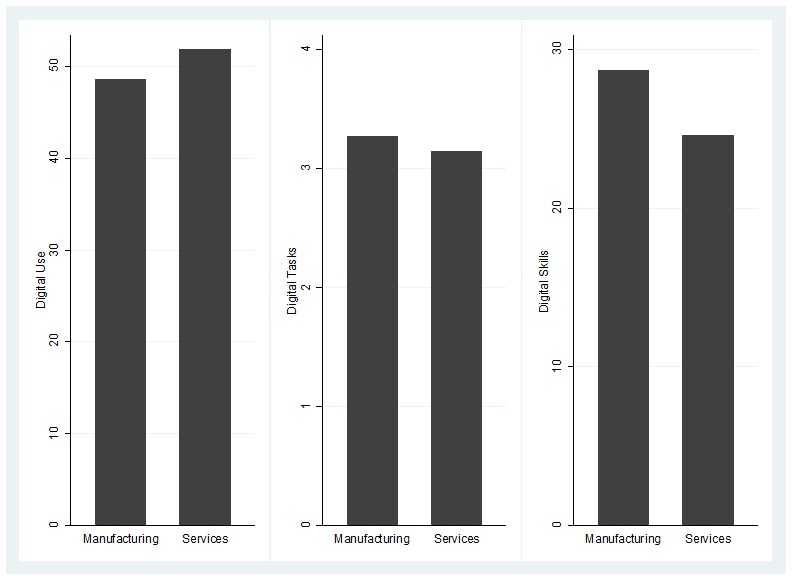
\includegraphics[width=\linewidth,height=0.8\textheight,keepaspectratio]{Figures/1_digital_sector.jpg}
\end{frame}

\begin{frame} 
\frametitle{Routine indices by sector}
\centering
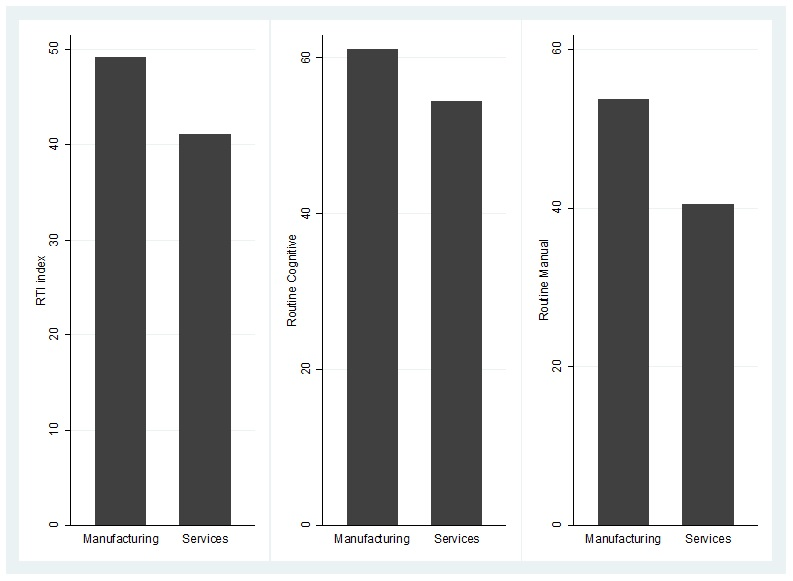
\includegraphics[width=\linewidth,height=0.8\textheight,keepaspectratio]{Figures/2_routine_sector.jpg}
\end{frame}

\begin{frame}
\frametitle{Digital indices by skill groups}
\centering
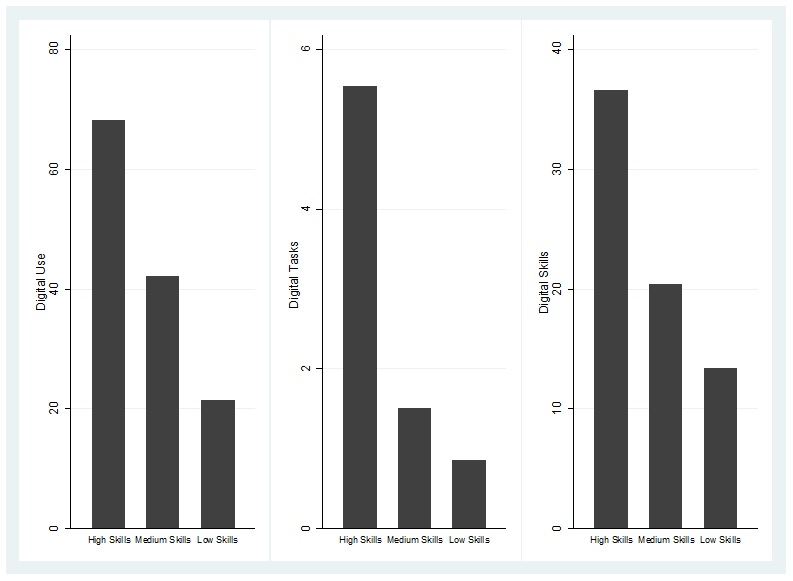
\includegraphics[width=\linewidth,height=0.8\textheight,keepaspectratio]{Figures/3_digital_skills.jpg}
\end{frame}

\begin{frame}
\frametitle{Routine indices by skill groups}
\centering
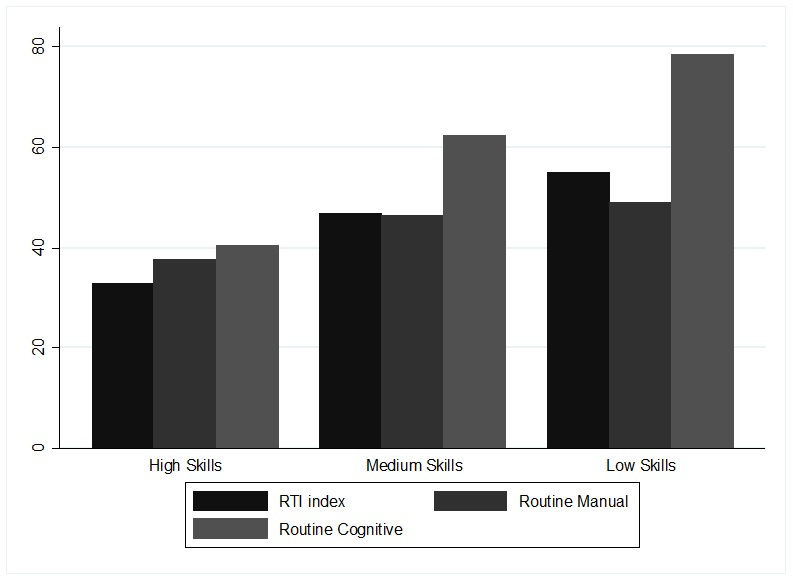
\includegraphics[width=\linewidth,height=0.8\textheight,keepaspectratio]{Figures/4_routine_skills.jpg}
\end{frame}

%\begin{frame}
%\frametitle{Correlation routine and digital indices}
%\centering
%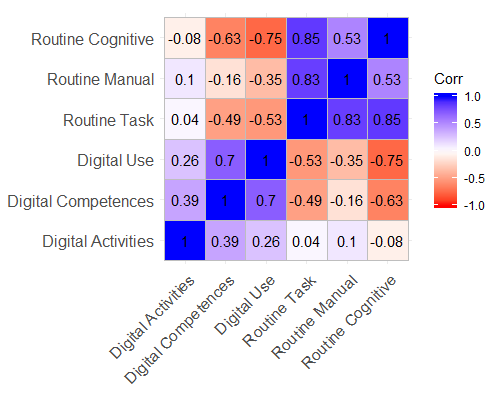
\includegraphics[width=\linewidth,height=0.8\textheight,keepaspectratio]{Figures/5_correlogram_indices.png}
%\end{frame}

%\begin{frame}
%\frametitle{Change in employment by skill group}
%\centering
%\includegraphics[width=\linewidth,height=0.8\textheight,keepaspectratio]{Figures/6_employment_sk%ills.jpg}
%\end{frame}

\begin{frame}
\frametitle{Change in employment by digital use}
\centering
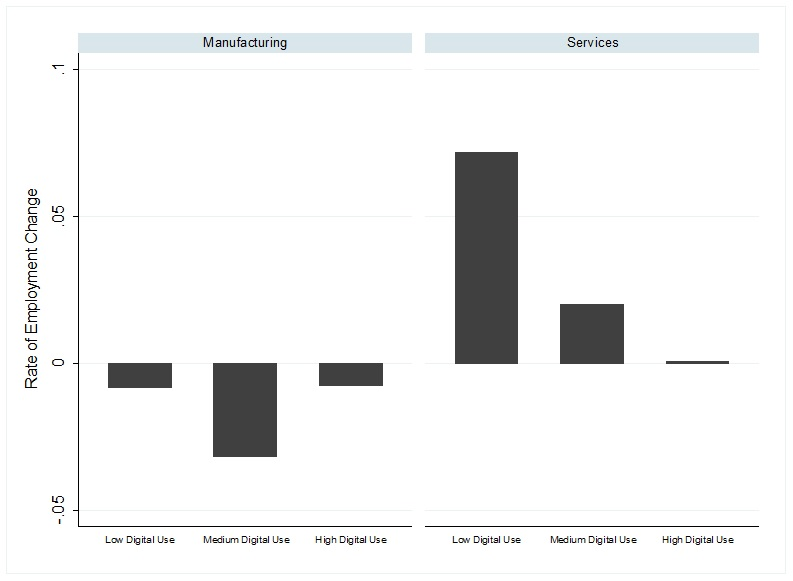
\includegraphics[width=\linewidth,height=0.8\textheight,keepaspectratio]{Figures/7_employment_digital_use.jpg}
\end{frame}

\begin{frame}
\frametitle{Change in employment by digital tasks}
\centering
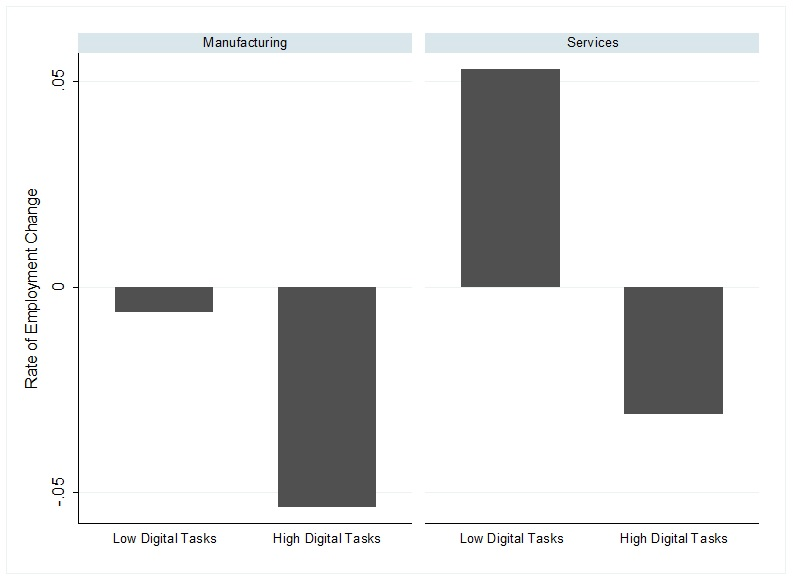
\includegraphics[width=\linewidth,height=0.8\textheight,keepaspectratio]{Figures/8_employment_digital_tasks.jpg}
\end{frame}

\begin{frame}
\frametitle{Change in employment by digital skills}
\centering
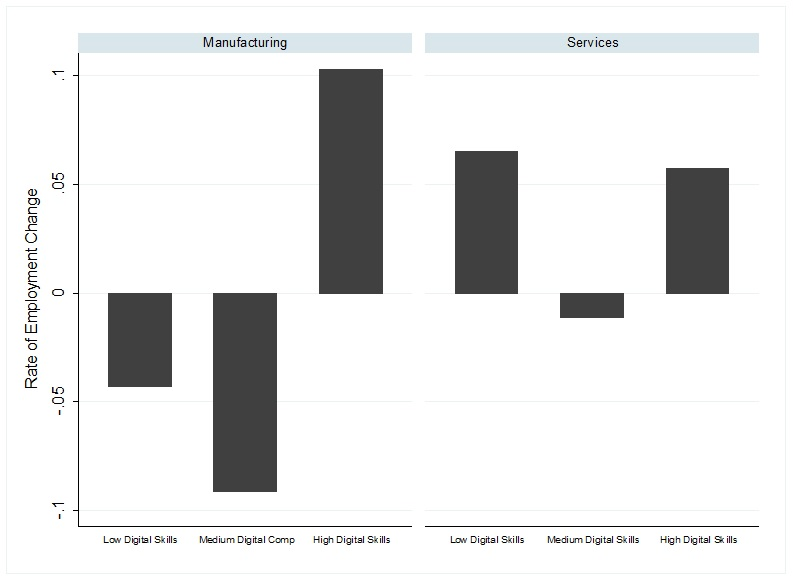
\includegraphics[width=\linewidth,height=0.8\textheight,keepaspectratio]{Figures/9_employment_digital_skills.jpg}
\end{frame}

\begin{frame}{Change by routineness and digitalization }
\tiny
\begin{table}[htbp]
  \centering
  \caption{Digital Use}
    \begin{tabular}{c|ccc|c}
          & DIGITAL USE<0.25 & 0.25 >DIGITAL USE < 0.75 & DIGITAL USE >0.75 &  \\
    \midrule
    RTI<0.25 & 2.19\% & -4.70\% & 5.97\% & -0.81\% \\
    0.25 >RTI < 0.75 & 4.98\% & 7.29\% & 3.49\% & 5.32\% \\
    RTI >0.75 & 1.92\% & -2.37\% & -16.15\% & -0.90\% \\
    \midrule
          & 2.87\% & -0.17\% & -0.56\% & 1.24\% \\
    \end{tabular}%
\end{table}%
% Table generated by Excel2LaTeX from sheet 'Foglio1'
\tiny
\begin{table}[htbp]
  \centering
  \caption{Digital Skills}
    \begin{tabular}{r|rrr|r}
          & DIGITAL SKILLS<0.25 & 0.25 >DIGITAL SKILLS < 0.75 & DIGITAL SKILLS >0.75 &  \\
    \midrule
    RTI<0.25 & -8.02\% & -5.70\% & 7.46\% & -0.81\% \\
    0.25 >RTI < 0.75 & 8.48\% & 3.64\% & 1.95\% & 5.32\% \\
    RTI >0.75 & 1.65\% & -10.56\% & 5.88\% & -0.90\% \\
    \midrule
          & 2.66\% & -3.46\% & 5.36\% & 1.24\% \\
    \end{tabular}%
  \label{tab:addlabel}%
\end{table}%

\tiny
\begin{table}[htbp]
  \centering
  \caption{Digital Tasks}
    \begin{tabular}{c|cc|c}
          & DIGITAL TASKS<0.50 & DIGITAL TASKS>0.50 &  \\
    \midrule
    RTI<0.25 & 0.67\% & -7.30\% & -0.81\% \\
    0.25 >RTI < 0.75 & 5.71\% & 3.74\% & 5.32\% \\
    RTI >0.75 & 0.87\% & -12.05\% & -0.90\% \\
    \midrule
          & 2.43\% & -4.67\% & 1.24\% \\
    \end{tabular}%
\end{table}%


\end{frame}



\section{Empirical strategy}

\begin{frame} 
\frametitle{Empirical strategy}

Combining the data from ILFS and ICP, we explore the relation (Weighted - OLS) between $\Delta N_{ij}$ changes in employment between 2011 and 2016 in occupation ($i$)--sector($j$) cells (ISCO 4-digit $\times$ NACE 1-digit) and:
\begin{itemize}
    \item $Digital_i$ occupational digital indices (use/skill/task);
    \item $RTI_i$ routine technical index:
    \item $X_{ij}$ occupation-sector controls:
    \begin{itemize}
        \item  the share of young employees (15-34 years old);
        \item the share of women; 
        \item the share of employees with temporary contracts;
        \item the share of part-time employees. 
    \end{itemize}
    \item $Y_i$: share of respondents in occupation $i$ who witnessed process innovation;
    \item $Z_j$: sector fixed effects;
    \item Robust Standard Errors.
\end{itemize}

\[\Delta N_{ij} = \alpha + \beta Digital_i + \delta RTI_i + \theta X_ij + \psi Y_i + Z_j + \varepsilon_{ij}\]
\[\Delta N_{ij} = \alpha + \beta Digital_i + \delta RTI_i + \gamma Digital_i \times RTI_i + \theta X_ij + \psi Y_i + Z_j + \varepsilon_{ij}\]
\end{frame}

\section{Results}
\begin{frame} 
\frametitle{Results}
\centering
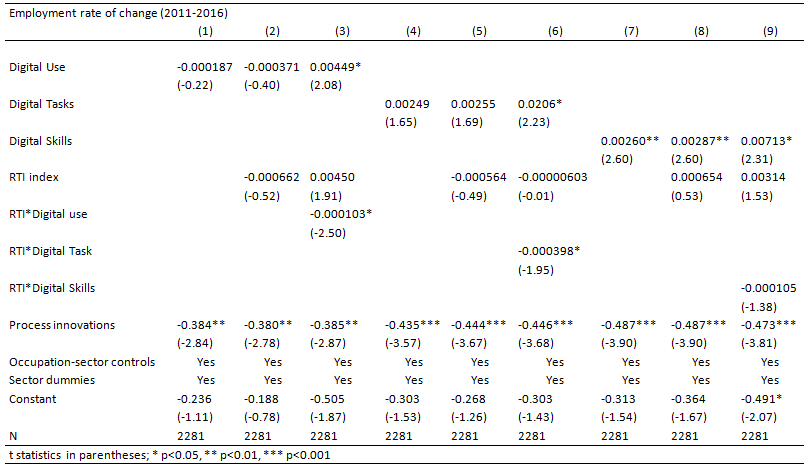
\includegraphics[width=\linewidth,height=0.8\textheight,keepaspectratio]{Figures/Results.png}
\end{frame}


\section{Conclusions}
\begin{frame} 
\frametitle{Conclusions}
%We contribute to the debate on the relationship between digital technologies and routine tasks on employment.


%We develop three distinct digital indicators of occupations (digital tasks, digital competences, digital use), and we calculate routineness (RTI) independently, using data provided by the INAPP-ISTAT survey on Italian occupations.
\smallskip

Results:

\begin{itemize}
    \item Complex relation between digitalization, routineness and skill levels: positive relation between digitalization and skills, negative between routineness and skill (descriptive evidence);
    \item Distinct effects between routineness and digitalization: highly digital professions see greater increase in employment (in manufacturing).
    \item Occupations using more digital tools - or with a high share of digital tasks - that are also highly routine tend to be penalized in employment terms.
\end{itemize}
\end{frame}

%\lastcredits{CREDITS}

\lastname{\textsl{Valeria Cirillo}}
\lastemail{\textsl{v.cirillo@inapp.org}}

\lastframe

\end{document}
